\documentclass[11pt]{article}
\usepackage[left=0.5in,right=0.5in,bottom=0.75in,top=0.75in]{geometry}

% Packages
\usepackage{amsmath}
\usepackage{amssymb}
\usepackage{amsthm}
\usepackage{graphicx}
\graphicspath{{code/out/}}
\usepackage{natbib}
\usepackage{hyperref}
\hypersetup{colorlinks=true, citecolor=black, linkcolor=., urlcolor=cyan}
\usepackage[font = small]{caption}
%\captionsetup{width=\linewidth}
\usepackage[shortlabels]{enumitem}
%\numberwithin{equation}{section}
\usepackage{booktabs}
\usepackage{algorithm}
\usepackage{algpseudocode}
\algdef{SxnE}[FOR]{For}{EndFor}[1]{\algorithmicfor\ #1 }
\usepackage{tikz}
\usetikzlibrary{tikzmark}
\usepackage{array} %% required by kableExtra if column_spec
\usepackage[normalem]{ulem}
\usepackage{appendix}
\usepackage{url}

% Theorems and algorithms
\newtheorem{thm}{Theorem}
\algnewcommand\algorithmicswitch{\textbf{switch}}
\algnewcommand\algorithmiccase{\textbf{case}}
\algnewcommand\algorithmicassert{\textbf{then }}
\algnewcommand\Assert[1]{\State \algorithmicassert #1}%
\algnewcommand\Assertif[2]{\State \textbf{if} #1 \algorithmicassert #2}
\algnewcommand\Assertelse[1]{\State \textbf{else} #1}
\algdef{SE}[SWITCH]{Switch}{EndSwitch}[1]{\algorithmicswitch\ #1}{\algorithmicend\ \algorithmicswitch}%
\algdef{SE}[CASE]{Case}{EndCase}[1]{\algorithmiccase\ #1}{\algorithmicend\ \algorithmiccase}%
\algtext*{EndSwitch}%
\algtext*{EndCase}%

% Macros
% Uppercase roman letters
\providecommand{\A}{\mathbf{A}}
\providecommand{\B}{\mathbf{B}}
\providecommand{\C}{\mathbf{C}}
\providecommand{\D}{\mathbf{D}}
\providecommand{\E}{\mathbf{E}}
\providecommand{\F}{\mathbf{F}}
\providecommand{\G}{\mathbf{G}}
\renewcommand{\H}{\mathbf{H}}
\providecommand{\I}{\mathbf{I}}
\providecommand{\J}{\mathbf{J}}
\providecommand{\K}{\mathbf{K}}
\providecommand{\L}{\mathbf{L}}
\providecommand{\M}{\mathbf{M}}
\providecommand{\N}{\mathbf{N}}
\providecommand{\O}{\mathbf{O}}
\renewcommand{\P}{\mathbf{P}}
\providecommand{\Q}{\mathbf{Q}}
\providecommand{\R}{\mathbf{R}}
\renewcommand{\S}{\mathbf{S}}
\providecommand{\T}{\mathbf{T}}
\providecommand{\U}{\mathbf{U}}
\providecommand{\V}{\mathbf{V}}
\providecommand{\W}{\mathbf{W}}
\providecommand{\X}{\mathbf{X}}
\providecommand{\Y}{\mathbf{Y}}
\providecommand{\Z}{\mathbf{Z}}

% Lowercase roman letters (c, d, u, v have to be treated special; see end)
\renewcommand{\a}{\mathbf{a}}
\renewcommand{\b}{\mathbf{b}}
\newcommand{\e}{\mathbf{e}}
\newcommand{\f}{\mathbf{f}}
\newcommand{\g}{\mathbf{g}}
\newcommand{\h}{\mathbf{h}}
\renewcommand{\i}{\mathbf{i}}
\renewcommand{\j}{\mathbf{j}}
\renewcommand{\k}{\mathbf{k}}
\renewcommand{\l}{\mathbf{l}}
\newcommand{\m}{\mathbf{m}}
\newcommand{\n}{\mathbf{n}}
\renewcommand{\o}{\mathbf{o}}
\newcommand{\p}{\mathbf{p}}
\newcommand{\q}{\mathbf{q}}
\renewcommand{\r}{\mathbf{r}}
\newcommand{\s}{\mathbf{s}}
\renewcommand{\t}{\mathbf{t}}
\newcommand{\w}{\mathbf{w}}
\newcommand{\x}{\mathbf{x}}
\newcommand{\y}{\mathbf{y}}
\newcommand{\z}{\mathbf{z}}
\let\origc\c
\DeclareRobustCommand\c{\ifmmode\mathbf{c}\else\expandafter\origc\fi}
\let\origd\d
\DeclareRobustCommand\d{\ifmmode\mathbf{d}\else\expandafter\origd\fi}
\let\origu\u
\DeclareRobustCommand\u{\ifmmode\mathbf{u}\else\expandafter\origu\fi}
\let\origd\v
\DeclareRobustCommand\v{\ifmmode\mathbf{v}\else\expandafter\origv\fi}

%% Roman letters with hats
\providecommand{\fhat}{\hat{f}}
\providecommand{\shat}{\hat{s}}
\providecommand{\yhat}{\hat{y}}
\providecommand{\bfhat}{\hat{\bf f}}
\providecommand{\bshat}{\hat{\mathbf{s}}}
\providecommand{\byhat}{\hat{\mathbf{y}}}

%% Roman letters with subscripts
\providecommand{\rj}{\mathbf{r}_{-j}}
\providecommand{\xj}{\mathbf{x}_{-j}}
\providecommand{\Xj}{\mathbf{X}_{-j}}

%% Roman letters with tildes
\providecommand{\rr}{\tilde{r}}
\providecommand{\xx}{\tilde{x}}
\providecommand{\yy}{\tilde{y}}
\providecommand{\zz}{\tilde{z}}
\providecommand{\brr}{\tilde{\mathbf{r}}}
\providecommand{\bxx}{\tilde{\mathbf{x}}}
\providecommand{\byy}{\tilde{\mathbf{y}}}
\providecommand{\bzz}{\tilde{\mathbf{z}}}
\providecommand{\XX}{\widetilde{\mathbf{X}}}
\providecommand{\WW}{\widetilde{\mathbf{W}}}
\providecommand{\ZZ}{\tilde{\mathbf{Z}}}

%% Script letters
\providecommand{\cA}{\mathcal{A}}
\providecommand{\cB}{\mathcal{B}}
\providecommand{\cC}{\mathcal{C}}
\providecommand{\cD}{\mathcal{D}}
\providecommand{\cE}{\mathcal{E}}
\providecommand{\cF}{\mathcal{F}}
\providecommand{\cG}{\mathcal{G}}
\providecommand{\cH}{\mathcal{H}}
\providecommand{\cI}{\mathcal{I}}
\providecommand{\cM}{\mathcal{M}}
\providecommand{\cN}{\mathcal{N}}
\providecommand{\cR}{\mathcal{R}}
\providecommand{\cS}{\mathcal{S}}
\providecommand{\cT}{\mathcal{T}}
\providecommand{\cU}{\mathcal{U}}
\providecommand{\cV}{\mathcal{V}}
\providecommand{\cW}{\mathcal{W}}
\providecommand{\cX}{\mathcal{X}}
\providecommand{\cY}{\mathcal{Y}}
\providecommand{\cZ}{\mathcal{Z}}

%% Greek letters
\providecommand{\ah}{\hat{\alpha}}
\providecommand{\ba}{\boldsymbol{\alpha}}
\providecommand{\bah}{\hat{\boldsymbol{\alpha}}}
\providecommand{\bb}{\boldsymbol{\beta}}
\providecommand{\bh}{\widehat{\beta}}
\providecommand{\bbh}{\widehat{\boldsymbol{\beta}}}
\providecommand{\bd}{\boldsymbol{\delta}}
\renewcommand{\dh}{\hat{\delta}}
\providecommand{\be}{\boldsymbol{\eta}}
\providecommand{\eh}{\hat{\eta}}
\providecommand{\beh}{\hat{\boldsymbol{\eta}}}
\providecommand{\eps}{\epsilon}
\providecommand{\veps}{\varepsilon}
\providecommand{\bep}{\boldsymbol{\epsilon}}
\providecommand{\bvep}{\boldsymbol{\varepsilon}}
\providecommand{\eph}{\hat{\epsilon}}
\providecommand{\beph}{\hat{\boldsymbol{\epsilon}}}
\providecommand{\gam}{\gamma}
\providecommand{\bg}{\boldsymbol{\gamma}}
\providecommand{\bgh}{\hat{\boldsymbol{\gamma}}}
\providecommand{\bG}{\boldsymbol{\Gamma}}
\providecommand{\gh}{\hat{\gamma}}
\providecommand{\bm}{\boldsymbol{\mu}}
\providecommand{\mh}{\hat{\mu}}
\providecommand{\bmh}{\hat{\boldsymbol{\mu}}}
\providecommand{\lam}{\lambda}
\providecommand{\Lam}{\Lambda}
\providecommand{\bl}{\boldsymbol{\lambda}}
\providecommand{\lh}{\hat{\lambda}}
\providecommand{\bL}{\boldsymbol{\Lambda}}
\providecommand{\bO}{\boldsymbol{\Omega}}
\providecommand{\bp}{\boldsymbol{\pi}}
\providecommand{\ph}{\hat{\pi}}
\providecommand{\bph}{\hat{\boldsymbol{\pi}}}
\providecommand{\bpsi}{\boldsymbol{\psi}}
\providecommand{\sh}{\hat{\sigma}}
\providecommand{\bS}{\boldsymbol{\Sigma}}
\providecommand{\bSh}{\hat{\boldsymbol{\Sigma}}}
\providecommand{\bt}{\boldsymbol{\theta}}
\renewcommand{\th}{\hat{\theta}}
\providecommand{\ts}{\theta^*}
\providecommand{\bth}{\hat{\boldsymbol{\theta}}}
\providecommand{\bts}{\boldsymbol{\theta}^*}
\providecommand{\bT}{\boldsymbol{\Theta}}
\providecommand{\btau}{\boldsymbol{\tau}}
\providecommand{\tauh}{\hat{\tau}}
\providecommand{\btauh}{\hat{\boldsymbol{\tau}}}
\providecommand{\bbj}{\boldsymbol{\beta}_{-j}}
\providecommand{\bbhj}{\widehat{\boldsymbol{\beta}}_{-j}}

%% Greek letters with tildes
\providecommand{\betat}{\widetilde{\beta}}
\providecommand{\bbjt}{\widetilde{\boldsymbol{\beta}}_{-j}}
\providecommand{\bbt}{\widetilde{\boldsymbol{\beta}}}
\providecommand{\etat}{\tilde{\eta}}
\providecommand{\bet}{\widetilde{\boldsymbol{\eta}}}
\providecommand{\lamt}{\tilde{\lambda}}
\providecommand{\mt}{\tilde{\mu}}
\providecommand{\bmt}{\tilde{\boldsymbol{\mu}}}
\providecommand{\nut}{\tilde{\nu}}
\providecommand{\thetat}{\tilde{\theta}}
\providecommand{\btt}{\tilde{\boldsymbol{\theta}}}

%% Operators
\renewcommand{\Pr}{\mathbb{P}}
\providecommand{\pr}{\textrm{Pr}}
\providecommand{\Ex}{\mathbb{E}}
\providecommand{\ex}{\textrm{E}}
\providecommand{\exh}{\widehat{\textrm{E}}}
\providecommand{\Var}{\mathbb{V}}
\providecommand{\var}{\textrm{Var}}
\providecommand{\varh}{\widehat{\textrm{Var}}}
\providecommand{\cov}{\textrm{Cov}}
\providecommand{\cor}{\textrm{Cor}}
\providecommand{\trace}{\textrm{tr}}
\providecommand{\rank}{\textrm{rank}}
\providecommand{\Norm}{\textrm{N}}
\providecommand{\Gmma}{\textrm{Gamma}}
\providecommand{\Beta}{\textrm{Beta}}
\providecommand{\Pois}{\textrm{Pois}}
\providecommand{\NBin}{\textrm{NegBin}}
\providecommand{\Unif}{\textrm{Unif}}
\providecommand{\Binom}{\textrm{Binom}}
\providecommand{\Bern}{\textrm{Bern}}
\providecommand{\Weib}{\textrm{Weibull}}
\providecommand{\Scx}{\textrm{Scaled-}\chi^2}
\providecommand{\Wish}{\textrm{Wishart}}
\providecommand{\Multinom}{\textrm{Multinom}}
\providecommand{\Dirch}{\textrm{Dir}}
\providecommand{\Exp}{\textrm{Exp}}
\providecommand{\diag}{\textrm{diag}}
\providecommand{\Tr}{^{\scriptscriptstyle\top}}

%% Statistical
\renewcommand{\l}{\ell}
\providecommand{\inP}{\overset{\textrm{P}}{\longrightarrow}}
\providecommand{\inAS}{\overset{\textrm{as\,}}{\longrightarrow}}
\providecommand{\inD}{\overset{\textrm{d}}{\longrightarrow}}
\providecommand{\inQM}{\overset{\textrm{qm\,}}{\longrightarrow}}
\providecommand{\adist}{\overset{\text{.}}{\sim}}
\providecommand{\AIC}{\textrm{AIC}}
\providecommand{\BIC}{\textrm{BIC}}
\providecommand{\CI}{\textrm{CI}}
\providecommand{\CV}{\textrm{CV}}
\providecommand{\FWER}{\textrm{FWER}}
\providecommand{\FDR}{\textrm{FDR}}
\providecommand{\FDRh}{\widehat{\textrm{FDR}}}
\providecommand{\fdr}{\textrm{fdr}}
\providecommand{\fdrh}{\widehat{\textrm{fdr}}}
\providecommand{\Fdr}{\textrm{Fdr}}
\providecommand{\Fdrh}{\widehat{\textrm{Fdr}}}
\providecommand{\GCV}{\textrm{GCV}}
\providecommand{\KL}{\textrm{KL}}
\providecommand{\LR}{\textrm{LR}}
\providecommand{\ME}{\textrm{ME}}
\providecommand{\MLE}{\textrm{MLE}}
\providecommand{\MSE}{\textrm{MSE}}
\providecommand{\MSPE}{\textrm{MSPE}}
\providecommand{\OLS}{\textrm{OLS}}
\providecommand{\PE}{\textrm{PE}}
\providecommand{\RSS}{\textrm{RSS}}
\providecommand{\SNR}{\textrm{SNR}}
\providecommand{\SE}{\textrm{SE}}
\providecommand{\SD}{\textrm{SD}}
\providecommand{\OR}{\textrm{OR}}
\providecommand{\RR}{\textrm{RR}}
\providecommand{\df}{\textrm{df}}
\providecommand{\odds}{\textrm{odds}}
\providecommand{\loglik}{\textrm{loglik}}
\providecommand{\logit}{\textrm{logit}}
\providecommand{\const}{\textrm{constant}}

% Fisher/observed information
\usepackage[scr=boondox]{mathalpha}
\providecommand{\oI}{\boldsymbol{\mathcal{I}}}
\providecommand{\oV}{\boldsymbol{\mathcal{V}}}

\makeatletter
\@ifpackagelater{mathalpha}{2021/01/01}{%
\providecommand{\fI}{\mathbfscr{I}}
\providecommand{\fV}{\mathbfscr{V}}
}{%
\providecommand{\fI}{\mathbscr{I}}
\providecommand{\fV}{\mathbscr{V}}
}
\makeatother

% Independence
\providecommand{\iid}{\overset{\text{iid}}{\sim}}
\providecommand{\ind}{\perp\!\!\!\perp}
\providecommand{\IID}{\overset{\scriptscriptstyle \ind}{\sim}}

%% Mathematical
\providecommand{\one}{\mathbf{1}}
\providecommand{\zero}{\mathbf{0}}
\providecommand{\intii}{\int_{-\infty}^{\infty}}
\providecommand{\real}{\mathbb{R}}
%%\providecommand{\Real}{\mathds{R}} %% Requires dsfonts
\providecommand{\dl}{d_-}
\providecommand{\dr}{d_+}
\providecommand{\sign}{\textrm{sign}}
\providecommand{\given}{\,\vert\,}
\providecommand{\abs}[1]{\left\lvert#1\right\rvert}
\providecommand{\sabs}[1]{\lvert#1\rvert}
\providecommand{\norm}[1]{\lVert#1\rVert}
\providecommand{\bignorm}[1]{\left\lVert#1\right\rVert}
\providecommand{\gl}{\prec}
\providecommand{\gle}{\preceq}
\providecommand{\gg}{\succ}
\providecommand{\gge}{\succeq}
\DeclareMathOperator*{\argmin}{\arg\min}
\DeclareMathOperator*{\argmax}{\arg\max}
\providecommand{\pf}[2]{\frac{\partial #1}{\partial #2}}

%% Equations
\providecommand{\al}[2]{\begin{align}\label{#1}#2\end{align}}
\providecommand{\as}[1]{\begin{align*}#1\end{align*}}
\providecommand{\als}[2]{\begin{align}\label{#1}\begin{split}#2\end{split}\end{align}}
\providecommand{\tcirc}[1]{\raisebox{.5pt}{\textcircled{\raisebox{-.9pt} {#1}}}}

% Other
\providecommand{\note}[1]{\textcolor{red}{#1}}
\providecommand{\MAF}{\textrm{MAF}}
\providecommand{\cvr}{\textrm{Cover}}


% Notes to each other
\newcommand{\pb}[1]{\textcolor{red}{#1}}
\newcommand{\logan}[1]{\textcolor{blue}{#1}}
\newlength{\li} \setlength{\li}{12pt}
\newcommand{\singlespace}{\baselineskip 1.1\li}

% Define abstract environment
\renewcommand{\abstract}[1]{
 \centerline{
 \begin{minipage}{0.7\linewidth}
 \hrule
 \vskip 0.1in
  \begin{center}
    {\bf Abstract}
  \end{center}
  #1
 \vskip 0.1in
 \hrule
 \end{minipage}}
 \vskip 0.3in}

% Title/author/date
\title{A New Perspective on High Dimensional Confidence Intervals}
\author{
  Logan Harris\\Department of Biostatistics\\University of Iowa
  \and
  Patrick Breheny\\Department of Biostatistics\\University of Iowa
}
\date{\today}


\begin{document}

\maketitle

\abstract{
  Classically, confidence intervals are required to have consistent coverage across all values of the parameter. However, this will inevitably break down if the underlying estimation procedure is biased. For this reason, many efforts have focused on debiased versions of the lasso for interval construction. In the process of debiasing, however, the connection to the original estimates are often obscured. In this work, we offer a different perspective focused on average coverage in contrast to individual coverage. This perspective results in confidence intervals that better reflect the original assumptions, as opposed to debiased intervals, which often do not even contain the original lasso estimates. To this end we propose a method based on the Relaxed Lasso that gives approximately correct average coverage and compare this to debiased methods which attempt to produce correct individual coverage. With this new definition of coverage we also briefly revisit the bootstrap, which Chatterjee and Lahiri (2010) showed was inconsistent for lasso, but find that it fails even under this alternative coverage definition.

}

\begin{figure}[htb!]
  \begin{center}
  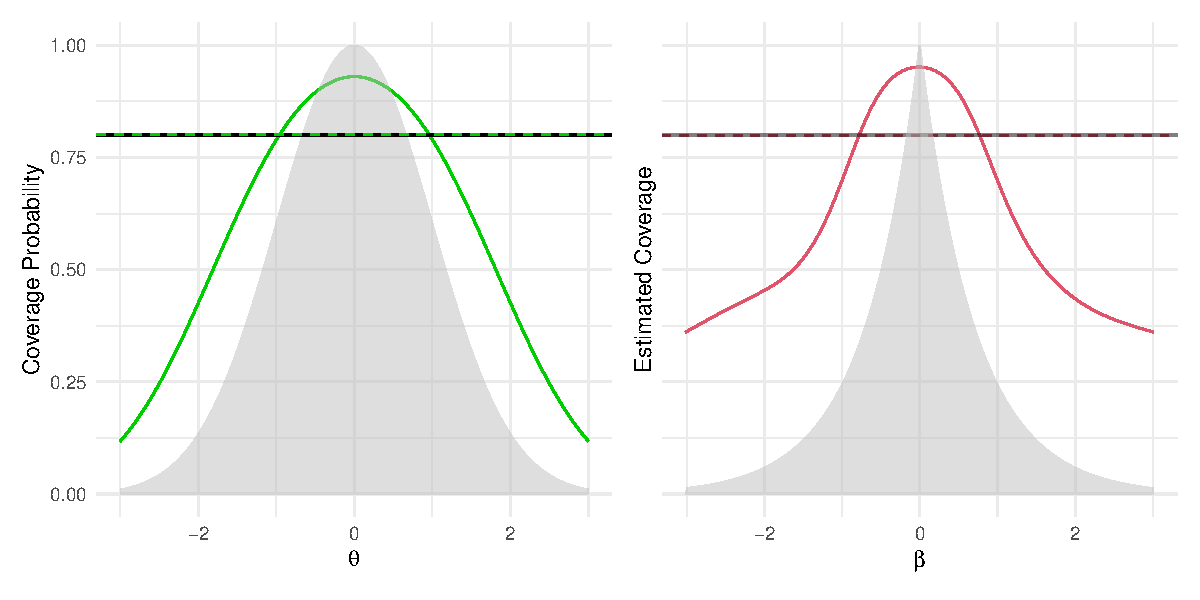
\includegraphics[width=0.8\linewidth]{figure1}
  \caption{\label{Fig:laplace} The left side of the figure provides coverage probabilities of Ridge CIs for a range of $\theta$ values as described in Section~\ref{Sec:difficulties}. The right side of the figure display results from the simulation described in Section~\ref{Sec:coverage}. For the right side of the figure, the fitted curve is from a Binomial GAM fit with coverage being modeled as a smooth function of $\beta$. The dashed line represent the average for the RL-P across all 1000 independently generated datasets and the solid black line indicates the nominal coverage rate. The shaded distribution in the background depicts the Laplace distribution the $\beta$s were drawn from. The analogous lines in the left side of the figure are exact calculations with the shaded normal in the background representing the prior.}
  \end{center}
\end{figure}

\begin{figure}[htb!]
  \begin{center}
  \includegraphics[width=0.7\linewidth]{figure2}
  \caption{\label{Fig:ridge_converge} Average coverages across p parameters (dashed lines) and estimated coverages as functions of $\beta$ (solid curves) for intervals constructed using a pairs bootstrap (Ridge Bootstrap) and a Bayesian posterior (Ridge). Full details of the simulation set up can be found in Section~\ref{Sec:boot-bias}.}
  \end{center}
\end{figure}

\begin{figure}[htb!]
  \begin{center}
  \includegraphics[width=0.8\linewidth]{figure3}
  \caption{\label{Fig:correlation_structure} This figure presents results for the simulation described in Section~\ref{Sec:correlation}. The violin plots are for the coverage rates across 1000 simulated datasets for the RL-P method and across three different levels of autoregressive correlation among the covariates, $\rho = 0 \text{ (no correlation)}, 0.5, 0.8$. For this simulation, p = 100, and the results for each level of correlation are presented across four different sample sizes, n = $\frac{1}{2}$p, p, 4p, 10p. The horizontal black line provides reference for the 80\% nominal coverage rate.}
  \end{center}
\end{figure}

\begin{table}[htb!]
  \centering
  \input{code/out/table1}
  \caption{\label{Tab:dist_beta} Results are from the simulation described in Section~\ref{Sec:distribution}. The nominal coverage rate is 80\%.}
\end{table}


\begin{figure}[htb!]
  \begin{center}
  \includegraphics[width=0.6\linewidth]{figure4.png}
  \caption{\label{Fig:beta_lambda_heatmap_laplace} The heatmap displays relative coverage for RL-P across a range of $\lambda$s per the simulation described in Section~\ref{Sec:lambda}. A Binomial GAM was used to estimate coverage as a smooth function of the $|\beta|$ and $\lam$. The x-axis for $\lambda$ is presented relative to $\lam_{\max}$ and the solid black lines indicate the center 95\% of $\lam_{\CV}$s over the 1000 simulations. The dashed black line indicates the median $\lambda_{\CV}$ and the blue line represents the value of $\lambda$ which provided coverage closest to that of nominal.}
  \end{center}
\end{figure}

\begin{figure}[htb!]
  \begin{center}
  \includegraphics[width=0.8\linewidth]{figure5}
  \caption{\label{Fig:highcorr} Provides results for simulation described in Section~\ref{Sec:Ridge}. The right plots show a single example of a intervals produced by Ridge (top) and RL-P (bottom) from one (randomly selected) of the 1000 datasets for the first 20 variables. The left plot summarizes the resulting CIs for the variables $A$, $B$, and $N1$ across the 1000 simulations. All 1000 CIs are plotted, sorted by their midpoint, with those colored red that did not contain contain the true coefficient value (indicated by the horizontal dashed gold line).}
  \end{center}
\end{figure}

\begin{figure}[htb!]
  \begin{center}
    \includegraphics[width=0.55\linewidth]{figure6}
    \caption{\label{Fig:laplace_comparison} Results are from the simulation described in Section~\ref{Sec:Comparison} and identical in setup to that of Section~\ref{Sec:coverage}. The fitted curves are from Binomial GAMs fit with coverage being modeled as a smooth function of $\beta$. The dashed lines represent the average coverage for each method across all 1000 independently generated datasets and the solid black line indicates the nominal coverage rate. The shaded distribution in the background depicts the Laplace distribution the $\beta$s were drawn from.}
  \end{center}
\end{figure}

\begin{figure}[htb!]
  \begin{center}
    \includegraphics[width=0.7\linewidth]{figure7}
    \caption{\label{Fig:laplace_other} Results are from the simulation described in Section~\ref{Sec:Comparison}. Each plot provides corresponding results for each of de-sparsified lasso, RL-P, and Selective Inference for three different sample sizes. The top provides violin plots of average coverages, the middle is a bar plot of the the median CI widths, and the bottom is a bar plot of the average run times, across all 1000 simulated datasets. The y limits have been truncated for the median width from 150 to 20.}
  \end{center}
\end{figure}

\begin{figure}[htb!]
  \begin{center}
    \includegraphics[width=0.9\linewidth]{figure8}
    \caption{\label{Fig:comparison_data_whoari} Confidence intervals produced by three different methods for all 66 variables in the WHO-ARI dataset described in Section~\ref{Sec:WHO-ARI}.}
  \end{center}
\end{figure}


\begin{table}[htb!]
  \centering
  \input{code/out/tableS1}
  \caption{Additional information on the results for Selective Inference in the simulation described in Section~\ref{Sec:Comparison}.}
\end{table}



\bibliographystyle{ims-nourl}
\bibliography{avg-cov}

\clearpage

\begin{appendices}
\renewcommand{\thesection}{Appendix~\Alph{section}}
\renewcommand{\thefigure}{Figure~\Alph{section}\arabic{figure}}
\renewcommand{\thetable}{Table~\Alph{section}\arabic{table}}
\renewcommand{\thealgorithm}{Algorithm~\Alph{section}\arabic{algorithm}}

% Reset counters manually at each new section
\makeatletter
\@addtoreset{figure}{section}
\@addtoreset{table}{section}
\@addtoreset{algorithm}{section}
\makeatother

% Remove default float prefixes in captions
\captionsetup[figure]{name={}}
\captionsetup[table]{name={}}
\floatname{algorithm}{} 
  
\section{Traditional Bootstrap Example}
\label{sec:boot-fail}

Figure~\ref{Fig:boot-fail} shows the coverage as a function of the value of $\beta$ (solid line) and the average coverage (dashed line) using a traditional pairs bootstrapping approach on the simulation setup described in Section~\ref{Sec:coverage}. Compare to the right side of Figure~\ref{Fig:laplace}.

\begin{figure}[hbtp]
  \begin{center}
  \includegraphics[width=0.7\linewidth]{figureA1}
  \caption{\label{Fig:boot-fail} Corresponds to the setup used in the right side of Figure~\ref{Fig:laplace}, but using a traditional bootstrapping approach.}
  \end{center}
\end{figure}

\clearpage

\section{Sampling from the Full Conditional Posterior}\label{Sup:A}

Here we assume $\X$ has been standardized s.t. $\x_j^T\x_j = n$. Define $\Q_{\hat{S}_j}$ as $\I - \X_{\hat{S}_j}(\X_{\hat{S}_j}^T \X_{\hat{S}_j})^{-1} \X_{\hat{S}_j}^T$, the projection matrix onto the features selected by the lasso. For $\beta_j$ conditional on the selected features

\as{
  \begin{aligned}
  L(\beta_j|\hat{S}_j) &\propto \exp(-\frac{\tilde{n}}{2\sigma^2}(\beta_{j}^2 - 2\tilde{\beta}_{j}\beta_{j})), \\
  \end{aligned}
}

where $\tilde{\beta}_j = (\x_j^T \Q_{\hat{S}_j} \x_j)^{-1} \x_j^T \Q_{\hat{S}_j} \y$ and $\tilde{n} = \x_j^T \Q_{\hat{S}_j} \x_j$.

The lasso can be formulated as a Bayesian regression model with a laplace (double exponential) prior. In this case, the prior for $\beta_j$ is proportional to $\exp(-\frac{\tilde{n} \lambda} {\sigma^2} \abs{\beta_j})$. This prior ensures that the meaning of $\lam$ is maintained.

With this the form of the full conditional posterior can be worked out as follows:
\as{
p(\beta_j | \hat{S}_j) &\propto \exp(-\frac{\tilde{n}}{2\sigma^2} (\beta_j^2 - 2\tilde{\beta}_j\beta_j)) \exp(-\frac{\tilde{n} \lambda} {\sigma^2} \abs{\beta_j}) \\
&= \exp(-\frac{\tilde{n}}{2\sigma^2} (\beta_j^2 - 2 \tilde{\beta}_{j}\beta_j +  2 \lambda \abs{\beta_j})) \\
&= \exp(-\frac{\tilde{n}}{2\sigma^2} (\beta_j^2 - 2(\tilde{\beta}_{j}\beta_j - \lambda \abs{\beta_j}))) \\
&=
\begin{cases}
\exp(-\frac{\tilde{n}}{2\sigma^2} (\beta_j^2 - 2(\tilde{\beta}_{j} + \lambda)\beta_j)), \text{ if } \beta_j < 0, \\
\exp(-\frac{\tilde{n}}{2\sigma^2} (\beta_j^2 - 2(\tilde{\beta}_{j} - \lambda)\beta_j )), \text{ if } \beta_j \geq 0 \\
\end{cases} \\
&\propto
\begin{cases}
C_{-} \exp\{-\frac{\tilde{n}}{2\sigma^2} (\beta_j - (\tilde{\beta}_j + \lambda))^2\}, \text{ if } \beta_j < 0, \\
C_{+} \exp\{-\frac{\tilde{n}}{2\sigma^2} (\beta_j - (\tilde{\beta}_j - \lambda))^2\}, \text{ if } \beta_j \geq 0 \\
\end{cases}
}
where $C_{-} = \exp(\tilde{\beta}_j \lambda \tilde{n}/\sigma^2)$ and $C_{+} = \exp(-\tilde{\beta}_j \lambda \tilde{n}/\sigma^2)$.

Note the piecewise defined posterior is made up of a kernel of two normal distributions. This can be leveraged and draws can be efficiently obtained through a mapping onto the respective normal distributions. To define this mapping, it helps to introduce a concept and some notation. First, the use of ``tails'' here refers to the entirety of a distribution between 0 and $\pm \infty$. That is, the lower tail is any part of the distribution below 0 and the upper tail is any part greater than 0, therefore $P(X \in lower \cup X \in upper) = 1$. Accordingly, we will let the tail probabilities in each of the two normals to transformed on to be denoted $Pr_{-}$ and $Pr_{+}$ respectively and the probability in each of the tails of the posterior, denoted $Post_{-}$ and $Post_{+}$ respectively. $Pr_{\pm}$ is trivial to compute with any statistical software. $Post_{\pm}$ is conceptually simple, although care must be taken to avoid numerical instability. With this notation in place, note that,
\as{
p(\beta_j | \hat{S}_j)  & \propto
\begin{cases}
C_{-} Pr_{-}, \text{ if } \beta_j < 0, \\
C_{+} Pr_{+}, \text{ if } \beta_j \geq 0\\
\end{cases}
} which implies that $Post_- = \frac{C_{-} Pr_{-}}{C_{-} Pr_{-} + C_{+} Pr_{+}}$ and similarly for $Post_+$. To avoid numerical instability, or rather to handle it properly when it is unavoidable, we will work on the $\log$ scale. This works well for most of the problem, but computation of $Post_-$ and $Post_+$ need something a bit more since, for example, $\log(Post_-) = \log(C_{-}Pr_{-}) - \log(C_{-} Pr_{-} + C_{+} Pr_{+})$. That is, the denominator still must be computed then the $\log$ taken which does not allow operating on the $\log$ scale to fully address potential numerical instability. Instead, let $\ell_{-} := \log C_{-} + \log Pr_{-}, \ell_{+} := \log C_{+} + \log Pr_{+}$, and $\Delta := \ell_{-} - \ell_{+}$, then $\log(Post_-)$ can be computed with $\Delta - \log\bigl(1 + \exp(\Delta)\bigr)$. This still doesn't completely address the issue, however, if $\exp(\Delta)$ is infinite then $C_-Pr_- >> C_+Pr_+$ and $\log(Post_-) \approx 0$ which means $Post_- \approx 1$ (equivalently $Post_+ \approx 0$).

With these values, we can compute the quantile by mapping the corresponding probability $p$ for the posterior onto the probability $p^*$ for the corresponding normals. Which normal the quantile of interest ultimately comes from is determined based on $Post_{\pm}$. If $p \leq Post_{-}$, then $p$ would be mapped onto the negative normal. If $p > Post_{-}$, then $p$ would be mapped onto the positive normal.  For example, if $Post_{+} = 0.98$ and $p = 0.1$ then $p$ would be mapped onto the positive normal. The transformation to map a given probability from the posterior depends on which tail the quantile resides in on the posterior (equivalently which normal it is being mapped to, the positive or negative). This map is simply:

\as{
p^* &= p \times (Pr_{\pm} / Post_{\pm}) \\
}


Once the respective probability is mapped, one can simply use the inverses of the normal CDF that the probability was mapped to. That being said, there is a nuance worth pointing out. When transforming the probabilities, the step to determine which tail the respective quantile comes from occurs first. With this, the probability should be adjusted so that it refers to the probability between the quantile of interest and the respective tail. After this, then the transformation can be applied. These steps are summarized in Algorithm~\ref{alg:quantile}.

\begin{algorithm}
\caption{Compute Quantile for RL-P Laplace-Normal Distribution}
\label{alg:quantile}
\begin{algorithmic}[1]
  \Require
    $\tilde{\beta}_j,\;\sigma^2,\;\tilde{n};\lambda,\;p$ \Comment{mean, variance, sample size, penalty, target significance level}
  \Statex
  \State // 1. Compute prior mass for negative and positive regions (on log‐scale)
  \State $Pr_{-} \gets \Phi\bigl(0;\,\tilde{\beta}_j + \lambda,\;\tfrac{\sigma^2}{\tilde{n}}\bigr)$
  \State $Pr_{+} \gets 1 - \Phi\bigl(0;\,\tilde{\beta}_j - \lambda,\;\tfrac{\sigma^2}{\tilde{n}}\bigr)$
  \Statex
  \State // 2. Compute posterior weights $Post_{-},\,Post_{+}$ with log‐scale stabilization
  \State $\ell_{-} \gets \log C_{-} + \log Pr_{-}$
  \State $\ell_{+} \gets \log C_{+} + \log Pr_{+}$
  \State $\Delta \gets \ell_{-} - \ell_{+}$
  \If{$\exp(\Delta) = \infty$}
    \State $\log Post_{-} \gets 0$  \Comment{since $C_-Pr_- \gg C_+Pr_+$}
  \Else
    \State $\log Post_{-} \gets \Delta - \log\bigl(1 + \exp(\Delta)\bigr)$
  \EndIf
  \State $Post_{-} \gets \exp(\log Post_{-})$
  \State $Post_{+} \gets 1 - Post_{-}$
  \Statex
  \State // 3. Invert CDF on the appropriate component
  \If{$p \le Post_{-}$}
    \State $w \gets \dfrac{Pr_{-}}{Post_{-}}$
    \State $q \gets \Phi^{-1}\bigl(p \,w;\;\tilde{\beta}_j + \lambda,\;\tfrac{\sigma^2}{n}\bigr)$
  \Else
    \State $w \gets \dfrac{Pr_{+}}{Post_{+}}$
    \State $q \gets \Phi^{-1}\!\Bigl(1 - (1-p)\,w;\;\tilde{\beta}_j - \lambda,\;\tfrac{\sigma^2}{n}\Bigr)$
  \EndIf
  \State \Return $q$
\end{algorithmic}
\end{algorithm}

\clearpage

\section{Coverage Behavior Under Alternative Sample Sizes}\label{Sup:alt_ns}

Figure~\ref{Fig:coverage_by_n} displays coverage estimates as a smooth function of $\beta$ for three values of n: 50, 100, and 400 but otherwise uses the same setup as the simulation described in Section~\ref{Sec:coverage}.

\begin{figure}[hbtp]
  \begin{center}
  \includegraphics[width=0.6\linewidth]{figureC1}
  \caption{\label{Fig:coverage_by_n} The results displayed are from a simulation with the same set up as in Section~\ref{Sec:coverage} but with n set to three different values: 50, 100, 400. The fitted curves are from Binomial GAMs fit with coverage being modeled as a smooth function of $\beta$. The dashed lines represent the average coverages across all 1000 independently generated datasets and the solid black line indicates the 80\% nominal coverage rate.}
  \end{center}
\end{figure}

For $n = 50$, coverage is overconservative with the characteristic high coverage for values near zero and low coverage for larger values of $\beta$. However, As $n$ is increased to 100 then 400 the characteristic over coverage for small $\beta$ values and under coverage for large $\beta$ values lessens, largely attributable to $\lam_{\CV}$ being smaller.

\clearpage

\section{Selective Inference Intervals}\label{Sup:si_int_info}


\begin{table}[hb]
  \singlespace
  \centering
  \input{code/out/tableD1}
  \caption{Additional information on the results for Selective Inference in the simulation described in Section~\ref{Sec:Comparison}.}
  \label{Tab:selective_inference}
\end{table}


Because Selective Inference only provides intervals for the subset of parameters with nonzero coefficients, the results in Figures~\ref{Fig:laplace_comparison} are just for this subset. This is in contrast to the results for de-sparsified lasso and RL-P which are over all parameters. The first two columns of Table~\ref{Tab:selective_inference} provide more details on the size of the lasso models selected by cross validation, and hence, on the number of intervals constructed. The first column indicates how many simulations (out of 1000) the intercept-only model was selected, in which case no intervals are produced. The second column gives the average number of selected parameters (inclusive of when none were selected). It is the subset of parameters represented by column 2 that are the results in Figures~\ref{Fig:laplace_comparison} are from.

For the intervals that were constructed, the third and fourth columns provide the number of simulations that had a infinite median width or any interval with an infinite width, respectively, features that were not evident in the right side of Figure~\ref{Fig:laplace_comparison}. Note that simulations where the null model was chosen by definition can not have intervals of infinite width.

\clearpage


\section{MCP Example}\label{Sup:MCP}

\begin{table}[hbtp]
  \centering
  \input{code/out/tableE1}
  \caption{\label{Tab:epsilon_conundrum_coverage} Coverage rates by magnitude of $\beta$ for RL-P using both the lasso and the MCP penalty approximation applied to the Sparse 1 scenario described in Section~\ref{Sec:distribution}. The nominal coverage rate is 80\%. }
\end{table}

The results here provide an example of a version of the RL-P method but with an approximation to the MCP penalty to obtain intervals. The MCP penalty closely resembles that of the lasso near zero but eventually levels out to a constant penalty for larger values of $\beta$ unlike the lasso which applies a penalty proportional to the magnitude of $\beta$. Note that although $\beta$s with intermediate magnitudes are still under covered (albeit with coverage notably higher than RL-P lasso), that the largest $\beta$s have coverage at nearly 70\%, over doubling the coverage of the RL-P lasso.

\clearpage

\section{Additional Details on Bootstrap Bias}\label{Sup:proof}

\begin{figure}[htb!]
  \begin{center}
    \includegraphics[width=0.7\linewidth]{figureF1}
    \caption{\label{Fig:ridge_converge} Average coverages across p parameters (dashed lines) and estimated coverages as functions of $\beta$ (solid curves) for intervals constructed using a pairs bootstrap (Ridge Bootstrap) and a Bayesian posterior (Ridge Posterior). Full details of the simulation set up can be found in Section~\ref{Sec:boot-bias}.}
  \end{center}
\end{figure}

We continue with a simple proof of the additional bias introduced by bootstrapping in one and two dimensional settings starting first with Ridge regression and then the lasso. After these simple proofs, we provide a simulation that helps generalize this issue to high dimensional settings. Note that here the goal is to provide an intuitive understanding of the issue. Others have already proved this issue more generally \citep{karoui2016, clarté2024}, however, we feel that the lack of straight forward examples may be in part why the bootstrap is still a tool used for penalized regression in general.

Let $\frac{1}{n}x_1^Tx_1 = s_{11}$, and $s_{11}^*$ be the bootstrapped version of $s_{11}$. Furthermore more that $E_{boot}[s_{11}^*] = s_{11}$.

For Ridge, it can be shown that $E(\bh_1) = \frac{s_{11}}{s_{11} + \lam}\beta_1$, letting $g(s_{11}) = \frac{s_{11}}{s_{11} + \lam}$ note that:

$$
\begin{aligned}
g'(s_{11}) &= \lambda (s_{11} + \lam)^{-2} \\
g''(s_{11}) &= -2\lambda (s_{11} + \lam)^{-3} < 0
\end{aligned}
$$

Thus by Jensen's inequality we have,

$$
E_{boot}[g(s_{11}^*)] \leq g(E_{booot}[s_{11}^*]) = g(s_11).
$$

Multiplying by $\beta_1$ then gives,

$$
E_{boot}[\bh_1^*] = E_{boot}[g(s_{11}^*)]\beta_1 \leq g(s_{11})\beta_1 = E[\bh_1].
$$

That is, even in a single parameter setting, just due to the bootstrap variability of $s_{11}$ alone, we would expect bias in the bootstrapped estimate of $\beta_1$.

Now consider a two parameter setting where we assume $\beta_2 = 0$. Let $V = \frac{1}{n}\boldsymbol{X}^T\boldsymbol{X} = \begin{pmatrix} s_{11} & s \\ s & s_{22} \end{pmatrix}$.

Similarly here, one can find that

$$
\begin{aligned}
E[\hat{\beta}_1 | V, \lambda] &= \frac{s_{11}(s_{22} + \lambda) - s^2}{(s_{11} + \lambda)(s_{22} + \lambda) - s^2} \beta_1 \\
&= g(s_{11}, s_{22}, s)\beta_1
\end{aligned}
$$


Furthermore, with some patience, it is possible to work out the Hessian of $g$:

$$
H = \nabla^{2}g
= \frac{\lambda}{D^{3}}
  \begin{pmatrix}
    -2(s_{22}+\lambda)^{3} & -2(s_{22}+\lambda)s^{2} & 4(s_{22}+\lambda)^{2}s\\[6pt]
    -2(s_{22}+\lambda)s^{2} & -2s^{2}(s_{11}+\lambda) & 2(s_{11}+\lambda)(D+2s^{2})s\\[6pt]
     4(s_{22}+\lambda)^{2}s &  2(s_{11}+\lambda)(D+2s^{2})s & -2(s_{22}+\lambda)(A+3s^{2})
  \end{pmatrix}.
$$

Because $\lambda/D^{3}>0$, negative semidefiniteness of $H$ is equivalent to that of the scaled matrix $\tilde H = D^{3}H/\lambda$.

$$
\tilde H_{11} = -2(s_{22}+\lambda)^{3} < 0
$$
$\det\bigl(\tilde H_{[1:2,1:2]}\bigr)$:
$$
\begin{aligned}
\det\bigl(\tilde H_{[1:2,1:2]}\bigr) &= \det \begin{pmatrix}
  -2(s_{22}+\lambda)^{3} & -2(s_{22}+\lambda)s^{2}\\[4pt]
  -2(s_{22}+\lambda)s^{2} & -2s^{2}(s_{11}+\lambda)
\end{pmatrix}\\[8pt]
&= 4(s_{22}+\lambda)^{2}s^{2}D \geq 0 \\
\end{aligned}
$$

and

$$
\det(\tilde H) = -\,8\,\lambda\,(s_{22}+\lambda)^{3}s^{2}\,(s_{11}+\lambda)\,D \leq 0.
$$

As such, $H$ is negative‐semidefinite and consequently $g(s_{11},s_{22},s)$ is globally concave in all three arguments. Now, let $V^*$ be the bootstrapped version of V and note that $E_{boot}[(s_{11}^*, s_{22}^*, s^*)] = (s_{11}, s_{22}, s)$. By Jensen's inequality:

$$
E_{boot}[g(S^*)] \leq g(E_{boot}[S^*]) = g(S).
$$

Multiplying by $\beta_1$ then gives:

$$
E_{boot}[\hat{\beta}_1^*] = E_{boot}[g(S^*)]\beta_1 < g(S)\beta_1 = E[\hat{\beta}_1].
$$

A similar argument can be made with the lasso, however, the mathematical details become more involved. Whereas with ridge we started off assuming the true values, with lasso it is easier to work with assumed conditions on the lasso estimates themselves as they directly affect the KKT conditions. Starting with a single parameter set up, assume that $\bh_1 > 0$. Then,

$$
\begin{aligned}
\frac{1}{n}\x_1^T(\y - \x_1 \bh_1) &= \lambda \\
\bh_1 &= \frac{1}{ns_{11}}\x_1^T\y - \frac{\lambda}{s_{11}} \\
E[\bh_1] &= \beta_1 - \frac{\lambda}{s_{11}} \\
\end{aligned}
$$

Let $h(s_{11}) = - \frac{\lambda}{s_{11}}$, then

$$
\begin{aligned}
h'(s_{11}) &= \frac{\lambda}{s_{11}^2}, \\
h''(s_{11}) &= \frac{-2\lambda}{s_{11}^3}  < 0\\
\end{aligned}
$$

and $h(s_{11})$ is therefore concave. So by Jensen's inequality

$$
\begin{aligned}
E_{boot}[h(s_{11}^*)] \leq h(E_{booot}[s_{11}^*]) = h(s_11).
\end{aligned}
$$

Adding $\beta_1$ then gives,

$$
\begin{aligned}
E_{boot}[\bh_1^*] = \beta_1 + E_{boot}[h(s_{11}^*)] \leq \beta_1 + g(s_{11}) = E[\bh_1].
\end{aligned}
$$

Now consider a two parameter setting. If we assume $\hat{\beta}_1 > 0$ and $\hat{\beta}_2 = 0$, bias can only be guaranteed when $\beta_2 = 0$. This boils down to the same details as the single parameter case we just considered. If both $\hat{\beta}_1$ and $\hat{\beta}_2$ are assumed positive, we arrive at the following KKT conditions:

$$
\begin{aligned}
\frac{1}{n}\boldsymbol{X}^T\boldsymbol{X} \hat{\boldsymbol{\beta}} &= \frac{1}{n}\boldsymbol{X}^Ty - \lambda 1_2 \\
\end{aligned}
$$

Again, let $\boldsymbol{V} = \frac{1}{n}\boldsymbol{X}^T\boldsymbol{X} = \begin{pmatrix} s_{11} & s \\ s & s_{22} \end{pmatrix}$, then

$$
\begin{aligned}
\hat{\beta_1} = \frac{s_{22}(x_1^Ty- n\lambda) - s(x_2^Ty- n\lambda)}{n(s_{11}s_{22} - s^2)}
\end{aligned}
$$

and

$$
\begin{aligned}
E(\hat{\beta}|X) &= \beta_1 - \lambda\frac{s_{22} - s}{s_{11}s_{22} - s^2} \\
&= \beta_1 + h(s_{11}, s_{22}, s)
\end{aligned}
$$

Differentiation gives
$$
\nabla^{2}h \;=\; \frac{\lambda}{D^{3}}
\begin{pmatrix}
-2s_{22}^{2}(s_{22}-s) & -2s_{22}s^{2} & 4s_{22}^{2}s\\[6pt]
-2s_{22}s^{2} & -2s_{11}s^{2} & 2\,s_{11}s\bigl(D+2s^{2}\bigr)\\[6pt]
4\,s_{22}^{2}s & 2\,s_{11}s\bigl(D+2s^{2}\bigr) & -2s_{22}\bigl(s_{11}s_{22}-s^{2}+3s^{2}\bigr)
\end{pmatrix}.
$$


Leading (1×1) minor:
  $$
    H_{11} = -\frac{2\lambda s_{22}^{2}(s_{22}-s)}{D^{3}} < 0
  $$

Leading (2×2) minor:
  $$
    \det\bigl(H_{[1:2,1:2]}\bigr)
      = \frac{4\lambda^{2}s_{22}^{2}s^{2}D}{D^{6}} \geq 0.
  $$

Full determinant:
  $$
    \det(H)
      = -\frac{8\lambda^{3}\,s_{22}^{3}s^{2}s_{11}\,s_{11}D}{D^{9}} \leq 0.
  $$

The Hessian is negative‐semidefinite.  Therefore the map $g(s_{11},s_{22},s)$ is jointly concave, and multivariate Jensen's inequality implies
$$
E_{\text{boot}}\bigl[\hat\beta_{1}^{*}\bigr]
  \;\le\; E\bigl[\hat\beta_{1}\mid X,\,z_{1}=z_{2}=+1\bigr],
$$
so the bootstrap mean of $\hat\beta_{1}$ sits strictly closer to zero than the original estimate whenever both fitted coefficients are positive. Note that in each of these settings a common thread is that the curvature, which affects the amount of bias introduced by the bootstrap is heavily dependent on $\lambda$. Thus, the larger $\lambda$ is the more the bootstrap will be biased. We also see in the two parameter setting that the correlation between features has a considerable role in the curvature. How much each of these contribute to the bootstrap bias is problem dependent, however, our exploration, such as the example we provide next, suggests that $\lambda$ is likely the larger influencer in general. That said, full exploration is outside the scope of this work, but could be explored by considering the eigenvalues for the hessians above under various scenarios.

How does this extend to high dimensions? To answer this question, we consider the following simulation study.

In order to increase interpretability, we consider a simplified scenario here. Consider a set up with $n = p = 100$ where there is 1 true non-null variable, $A$ s.t. $\beta_A = 2$ that is correlated with a null variable $B$ with $\rho = 0.5$. All other variables are generated independent of $A$ and each other. For this set up, $A$ is always selected to be in the model, both with the original data and for all bootstrap replications at $\lam_{CV}$. This is important as decomposing the bias is more complicated for variables that are not selected to be in the model.

Note, the bias for $\bh_j \neq 0$ is $\frac{1}{n}\x_j^T \epsilon + \frac{1}{n}\x_j^T \X_{-j}(\bb^*_{-j} - \bbh_{-j}) + \lam$. We can break this down further to apply to the scenario outlined above. $Bias_A = \frac{1}{n}\x_A^T \epsilon + \frac{1}{n}\x_A^T \x_{B}(\beta^*_{B} - \bh_{B}) + \frac{1}{n}\x_A^T \X_{N}(\bb^*_{N} - \bbh_{N}) + \lam$. That is, we can decompose the bias into four parts. The first is the irreducible bias which comes from the chance correlation between $\x_A$ and the errors. The last is the bias directly introduced by the lasso penalty. The other two components attribute bias from the single $B$ variable and all 98 $N$ variables respectively. By taking the simulation set up in the previous paragraph and repeating it 1000 times and each time saving the bias attributable to each of the components, we can get an idea of the distribution of the bias components. More specifically, for each generated dataset, we can decompose the bias for the estimates from the original data as well as from the 1000 bootstrap replications. For the bootstrap replications, we can then save the mean bias. Figure~\ref{Fig:bias_decomp_single_B} shows a summary from doing just that. The top panel gives the densities of the mean bootstrap biases across the 1000 repetitions, the middle gives the densities for the biases on the original dataset across the 1000 repetitions, and the bottom give the densities of their paired differences. In this depiction, the contribution of $\lam$ is excluded. Additionally note here that a positive bias is used to indicated bias \emph{towards} zero.

\begin{figure}[hbtp]
    \begin{center}
    \includegraphics[width=\linewidth]{figureF2}
    \caption{\label{Fig:bias_decomp_single_B} n = p = 100, $\beta_A = 2$, $\beta_B = 0$, $\rho_{A,B} = 0.5$.  All other $\beta$s = 0 and  generated under independence}
    \end{center}
\end{figure}

While the derivation above suggests that increasing correlation is the main contributor to increased bootstrap bias, we see that it is actually the cumulative effect of the 98 N variables that drives the bias rather than the correlation with variable $B$. This has important implications in that even when overall correlations are low, that the sparsity in high dimensional settings is going to lead to a significant bootstrap bias. It is important to differentiate this bias and the bias inherent in the motivation for Section~\ref{Sec:IAC}. The framework put forth in Section~\ref{Sec:IAC} allows for the bias introduced by penalization which we are arguing is permissible in this newly suggested coverage framework, however, the additional bootstrap bias here is what inherently leads to the breakdown of the bootstrap even for average coverage.

\clearpage
\section{A note about stability selection}
\label{sec:stability}

It is no secret that bootstrapping lasso has fundamental issues. The related work in this manuscript is simply meant to show easy to comprehend details to this end. With these issues in mind, it is not common to see a traditional bootstrapping approach applied to the lasso for the purposes of interval construction. Rather, the popular use of resampling techniques for the lasso is in stability selection introduced by  \cite{Meinshausen2010}. However, here, we show that stability selection is still affected by bootstrap bias.

Consider the following set up. $n = 50$, $p = 500$, 4 $\beta$s contain signal: $\beta_{1-4} = (0.25, 0.5, 1, 2)$ and the rest are zero. $\X$ were generated independently from a $\Norm(0, 1)$. Finally, $\y$ was generated as $\y = \X\bb + \bvep$, where $\veps_i \iid N(0, 1)$. Using this data setup, stability selection was performed as outlined in Algorithm~\ref{alg:singlelambda}.

\begin{algorithm}[!ht]
\caption{Bootstrap Stability Selection at a \emph{single} CV‐chosen $\lambda$}
\label{alg:singlelambda}
\begin{algorithmic}[1]
\Require\ $R$ replicated data sets, $B$ bootstraps per data set,
          $p$ predictors
\Statex \textbf{Let:}
  $\mathbf A \in\{0,1\}^{R\times p}$, $\mathbf A^{\!*}\in[0,1]^{R\times p}$
%
\For{$i=1,\dots,R$}
  \State Generate $(\mathbf X,\mathbf y)$ from the data-generating process
  \State $\lambda_{\text{CV}}\leftarrow
         \operatorname*{arg\,min}_{\lambda}\text{CV‐Error}(\lambda)$
         \Comment{10-fold CV on $(\mathbf X,\mathbf y)$}
  \State Obtain lasso estimates at $\lambda_{\text{CV}}$
        and save
        $\mathbf A_{i,\cdot}\gets\bigl[\hat\beta(\lambda_{\text{CV}})\neq 0\bigr]$

  \State Initialise $\mathbf B^{\!*}\gets\mathbf 0_{B\times p}$
  \For{$b=1,\dots,B$}                        \Comment{pairs bootstraps}
     \State Draw indices $\mathcal I_b$ with replacement from $\{1,\dots,n\}$
     \State $(\mathbf X^{b},\mathbf y^{b})\gets
            (\mathbf X_{\mathcal I_b,\cdot},\mathbf y_{\mathcal I_b})$
     \State Fit lasso on $(\mathbf X^{b},\mathbf y^{b})$ at $\lambda_{\text{CV}}$
     \State $\mathbf B^{\!*}_{b,\cdot}\gets
            \bigl[\hat\beta^{\!*}(\lambda_{\text{CV}})\neq 0\bigr]$
  \EndFor
  \State $\mathbf A^{\!*}_{i,\cdot}\gets
         \dfrac1B\sum_{b=1}^{B}\mathbf B^{\!*}_{b,\cdot}$
\EndFor
\end{algorithmic}
\end{algorithm}

After we computed $\bar{\mathbf A}\gets\dfrac1R\sum_{i=1}^{R}\mathbf A_{i,\cdot}$,  \; $\bar{\mathbf A}^{\!*}\gets\dfrac1R\sum_{i=1}^{R}\mathbf A^{\!*}_{i,\cdot}$ and then compare $\bar{\mathbf A}$ (prob.\ of being selected in the original fit) with $\bar{\mathbf A}^{\!*}$ (expected bootstrap stability) to evaluate how well the inclusion probabilities mirror single-$\lambda$ selection behavior. The results are presented in Table~\ref{Tab:stability_selection}.

\begin{table}[hbtp]
  \centering
  \input{code/out/tableG1}
  \caption{\label{Tab:stability_selection} Results for simulation described in Section~\ref{sec:stability} showing that stability selection also suffers from bootstrap bias. Original selection(\%) provides the empirical selection probabilities for the 4 parameters while Bootstrap stability gives the bootstrap estimate for selection.}
\end{table}

Clearly, there is a fundamental bias for stability selection. That said, further exploration is necessary to understand if this contradicts the claims of \cite{Meinshausen2010} as they primarily focus on FDR control for finite sample problems like the one considered here.

Note, this implementation deviates from the proposed stability selection algorithm originally introduced by \cite{Meinshausen2010} in order to retain a connection to the bootstrap implementation in this manuscript, however, even when considering the entire lasso path fit on sub-bagged samples the bias remained largely the same.
                       
\end{appendices}

\end{document}
